\section{Methods}\label{sec:methods}
In this chapter, the methods for investigating a bridge design, verifying its structural safety and estimating its cost are introduced. In Section \ref{sec:met_ref} the Blennerhassett Island Bridge, as well as other reference bridges, are presented.
Section \ref{sec:met_str} describes the structural model which was used to calculate the effects for different load cases. The underlying assumptions are briefly specified and assessed. Further, an overview of the investigated load cases is given in Section \ref{sec:met_loads}. The determination of the self-equilibrium stress state is of critical importance. The designer can freely assign it to the structure, contrary to the load cases, whose effects are determined by the elastic response of the structure. Section \ref{sec:met_seq} describes different methods to obtain this state which also includes the determination of the arch shape. The limit states for the design criteria as well as the corresponding verifications are obtained in Section \ref{sec:met_ver}, combining the self-equilibrium stress state with the factored load cases. Based on these verifications, the cost of the investigated design is estimated in Section \ref{sec:met_cost}. The methods presented in this chapter are exemplified by the final design of the Blennerhassett Island Bridge according to the design drawings.

\subsection{Reference bridges} \label{sec:met_ref}

\newpage
\subsection{Structural modelling} \label{sec:met_str}
A defining feature of the Blennerhassett Island Bridge is the floating deck. It is supported only at the 13 floor beams and acts as an almost independent structural component. Compared to a composite deck, it causes a certain inefficiency in material use and the additional arrangement of many bearings. On the other hand, it allows for a replacement of the deck in the future and it simplifies the investigation of the flow of forces. It carries the loads over a span of 20 meters to the adjacent floor beams. There, the forces are mainly carried by the respective hanger pair and partially by the tie girder. This feature allows for a separation of the behaviour of the remaining network arch from the deck. As it is not the objective of this Thesis to investigate and optimise the deck system it is not further considered. The structural model of the network tied-arch bridge is therefore composed of the tie, the arch and the hangers. According to \citep{Smit}, the behaviour of the two planes of the arch can be considered decoupled from each other. Therefore, the behaviour of the arch is analysed in a single plane.\bigskip

Considering their slenderness, the arch and the tie can be accurately modelled as beam elements. Considering the low bending stiffness of the hangers, secondary effects cannot always be neglected. However, the comparison in Appendix \ref{Appendix_A_Hangers} showed that above \SI{100}{MPa} secondary effects are irrelevant for this cable geometry. Therefore, the hangers are modelled as beams with rotational end releases and neglecting their self-weight. Hence, the structure is analysed in the framework of two-dimensional and linear elastic beam statics. The structural analysis is conducted using a python package written by the author of this Thesis in an earlier project.\bigskip

The results are analysed in defined segments along the arch and the tie. On these segments, the maximum degree of compliance which will determine the cost of each segment is calculated individually. An overview of the Blennerhassett Island Bridge and its structural model with its segments are shown in Figs. \ref{fig:Blennerhassett2_a} and \ref{fig:fig:Blennerhassett2_b}.

\begin{figure}[H]
\centering
\begin{subfigure}{0.5\textwidth}
    \centering
    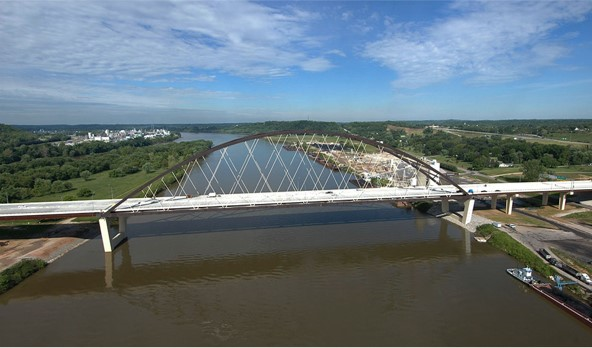
\includegraphics[width=0.9\textwidth]{overleaf/Pictures/Blennerhassett_2.jpg}
    \caption{Built structure}
    \label{fig:Blennerhassett2_a}
\end{subfigure}%
\begin{subfigure}{.5\textwidth}
    \centering
    \vspace*{0.67cm}
    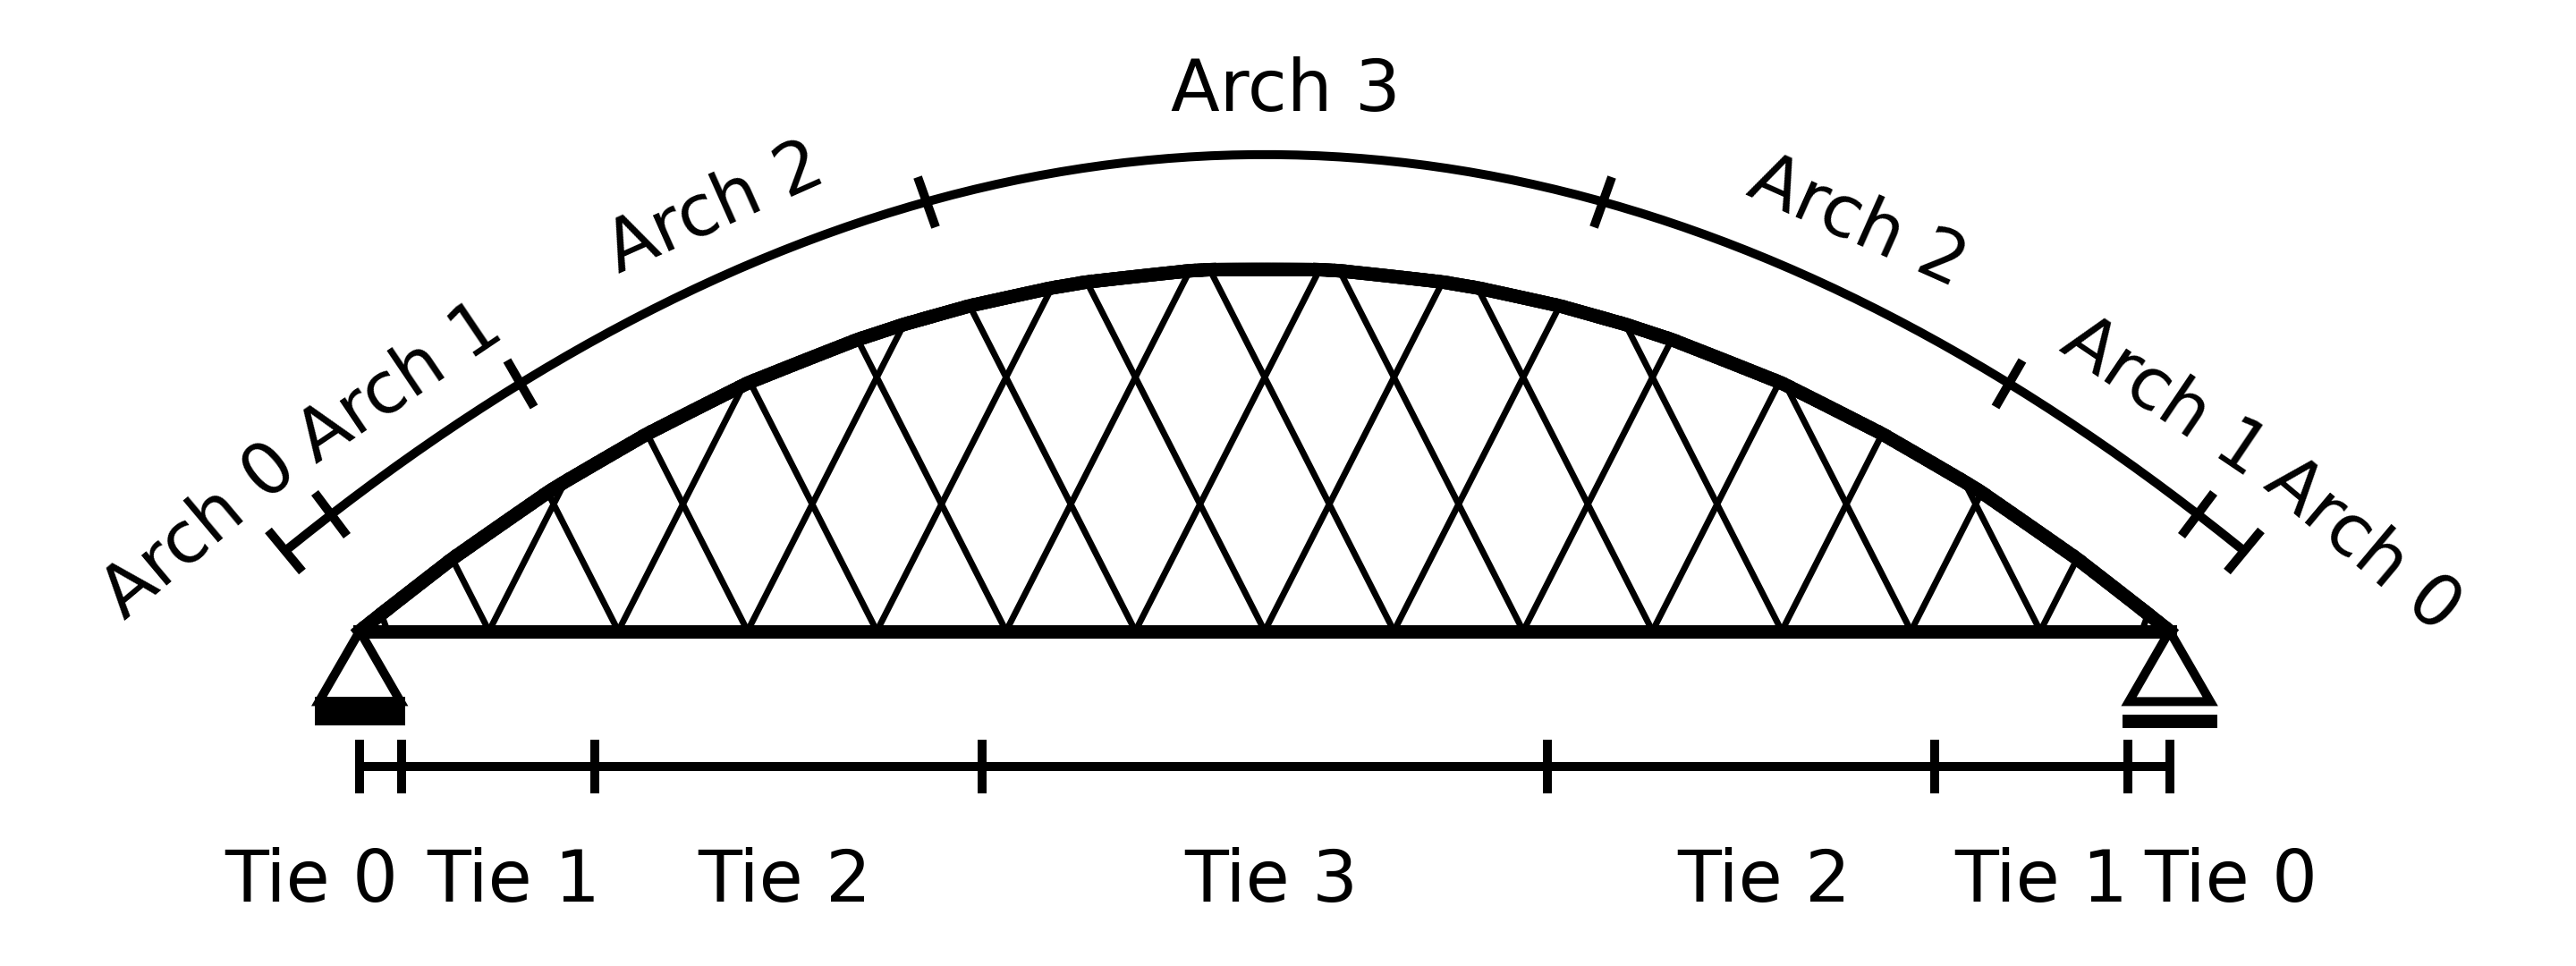
\includegraphics[width=0.9\textwidth]{illustrations/model overview/segments.png}
    \vspace*{0.67cm}
    \caption{Structural model and segments}
    \label{fig:fig:Blennerhassett2_b}
\end{subfigure}
\caption{Blennerhassett Island Bridge}
\label{fig:Blennerhassett2}
\end{figure}

The arch and the tie feature different cross-sections in the knuckle region, where the highest internal force effects are expected. The respective stiffnesses are up to twice as high as the stiffness of the field cross-sections, as presented in Table \ref{tab:cs_stiffnesses}. Additionally, there is also a web connecting the tie and the arch at the knuckle, as shown in Figure \ref{fig:knuckle_region}.

\begin{table}[H]
\caption{Cross-sectional stiffnesses}
\label{tab:cs_stiffnesses}
\centering
\begin{tabular}{lccc}
\hline
Segment & Normal stiffness & Bending stiffness & Shear stiffness \\
 & [\SI{}{MN}]   & [\SI{}{MNm^2}] & [\SI{}{MN}] \\ \hline
Arch 1 & \SI{77429}{} & \SI{31473}{} & \SI{79.1}{}\\
Arch 2 & \SI{65997}{} & \SI{28673}{} & \SI{63.4}{}\\
Arch 3-4 & \SI{61814}{} & \SI{28113}{} & \SI{42.7}{}\\
Tie 1 & \SI{77429}{} & \SI{31473}{} & \SI{76.2}{}\\
Tie 2 & \SI{65997}{} & \SI{28673}{} & \SI{56.6}{}\\
Tie 3-4 & \SI{61814}{} & \SI{28113}{} & \SI{45.8}{}\\
Hangers & 643 & - & - \\\hline
\end{tabular}
\end{table}

\begin{figure}[H]
    \centering
    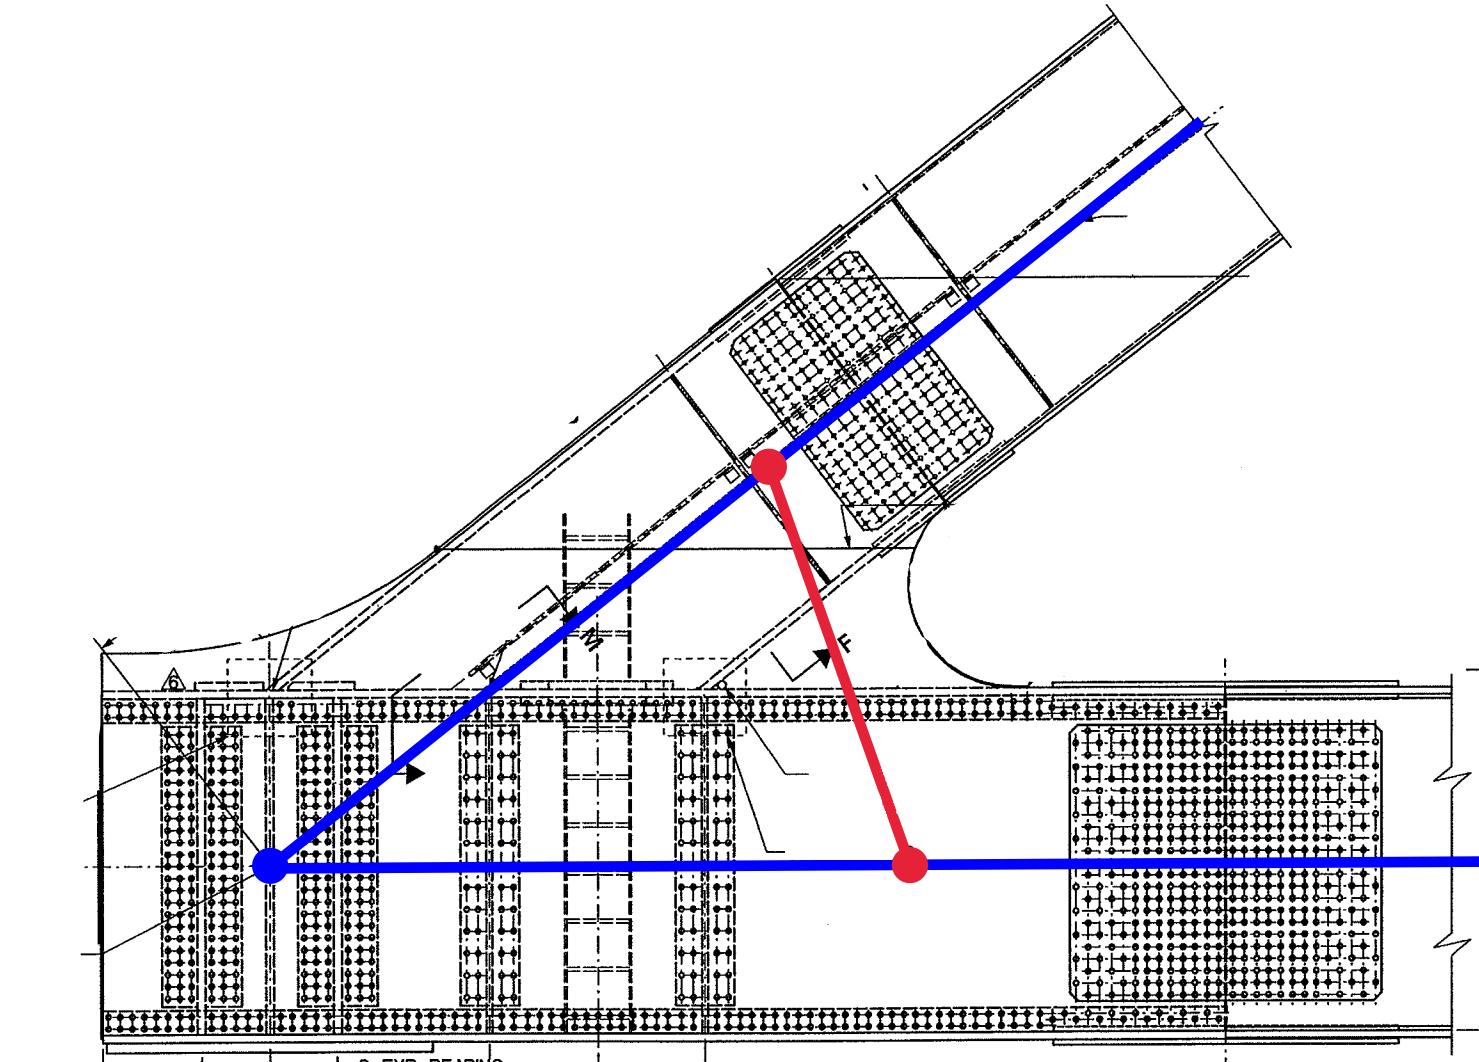
\includegraphics[width=0.8\textwidth]{overleaf/Pictures/Knuckle region.png}
    \caption{Plan and modelling of the knuckle region}
    \label{fig:knuckle_region}
\end{figure}

To judge the influence of these features on the internal force effects, the structure is analysed using different models. In the first model, the field cross-sections are used everywhere and also no web member is considered. In a second model, a web steel member with a cross-section of 0.127m x 1.067m is introduced. Additionally, the actual cross-sections are assigned to the arch and the tie in a third model. The effects under dead loads are compared region-wise between the three different models. The results are presented in Table []. [conclusion]

\newpage
\subsection{Load cases} \label{sec:met_loads}
The load cases relevant to this investigation are the dead loading (DL), the live loading (LL) and the wind loading (WS). The dead loading is further subdivided into the weight of the structural components (DC) and the weight of the future wearing surfaces and utilities (DW).

\subsubsection{Dead loading}
The dead loads for the Blennerhassett Island Bridge were derived from the estimated bridge quantities of the design drawings. The detailed derivation is given in Appendix [] and the final results are presented in Table \ref{tab:dead_loads}. The weight of the arch and the tie girder are constantly distributed along the respective elements. A particularly detailed weight distribution by assigning more weight to the stronger cross-sections near the knuckle is disregarded for. Also the weight of the lateral bracing is distributed along the entire arch for simplicity. The deck weight and its non-structural components make up for the main contribution to the dead loading. The weight of the deck, on the other hand, is applied as a concentrated force at the locations of the cross-girders. The weight of the hangers and its resulting bending moment is relatively small and neglected to facilitate some of the used methods. An illustration of all dead loads applied to the structural model is shown in Fig. \ref{fig:dead_loads}.

\begin{table}[H]
    \centering
    \begin{tabular}{lccccc}
        Component & Arch & Tie & Deck & Utilities & Unit \\ \hline
        Weight & 29.8 & 26.4 & 115.3 & 35.1 & \SI{}{kN/m}
    \end{tabular}
    \caption{Weight per component}
    \label{tab:dead_loads}
\end{table}

\begin{figure}[H]
    \centering
    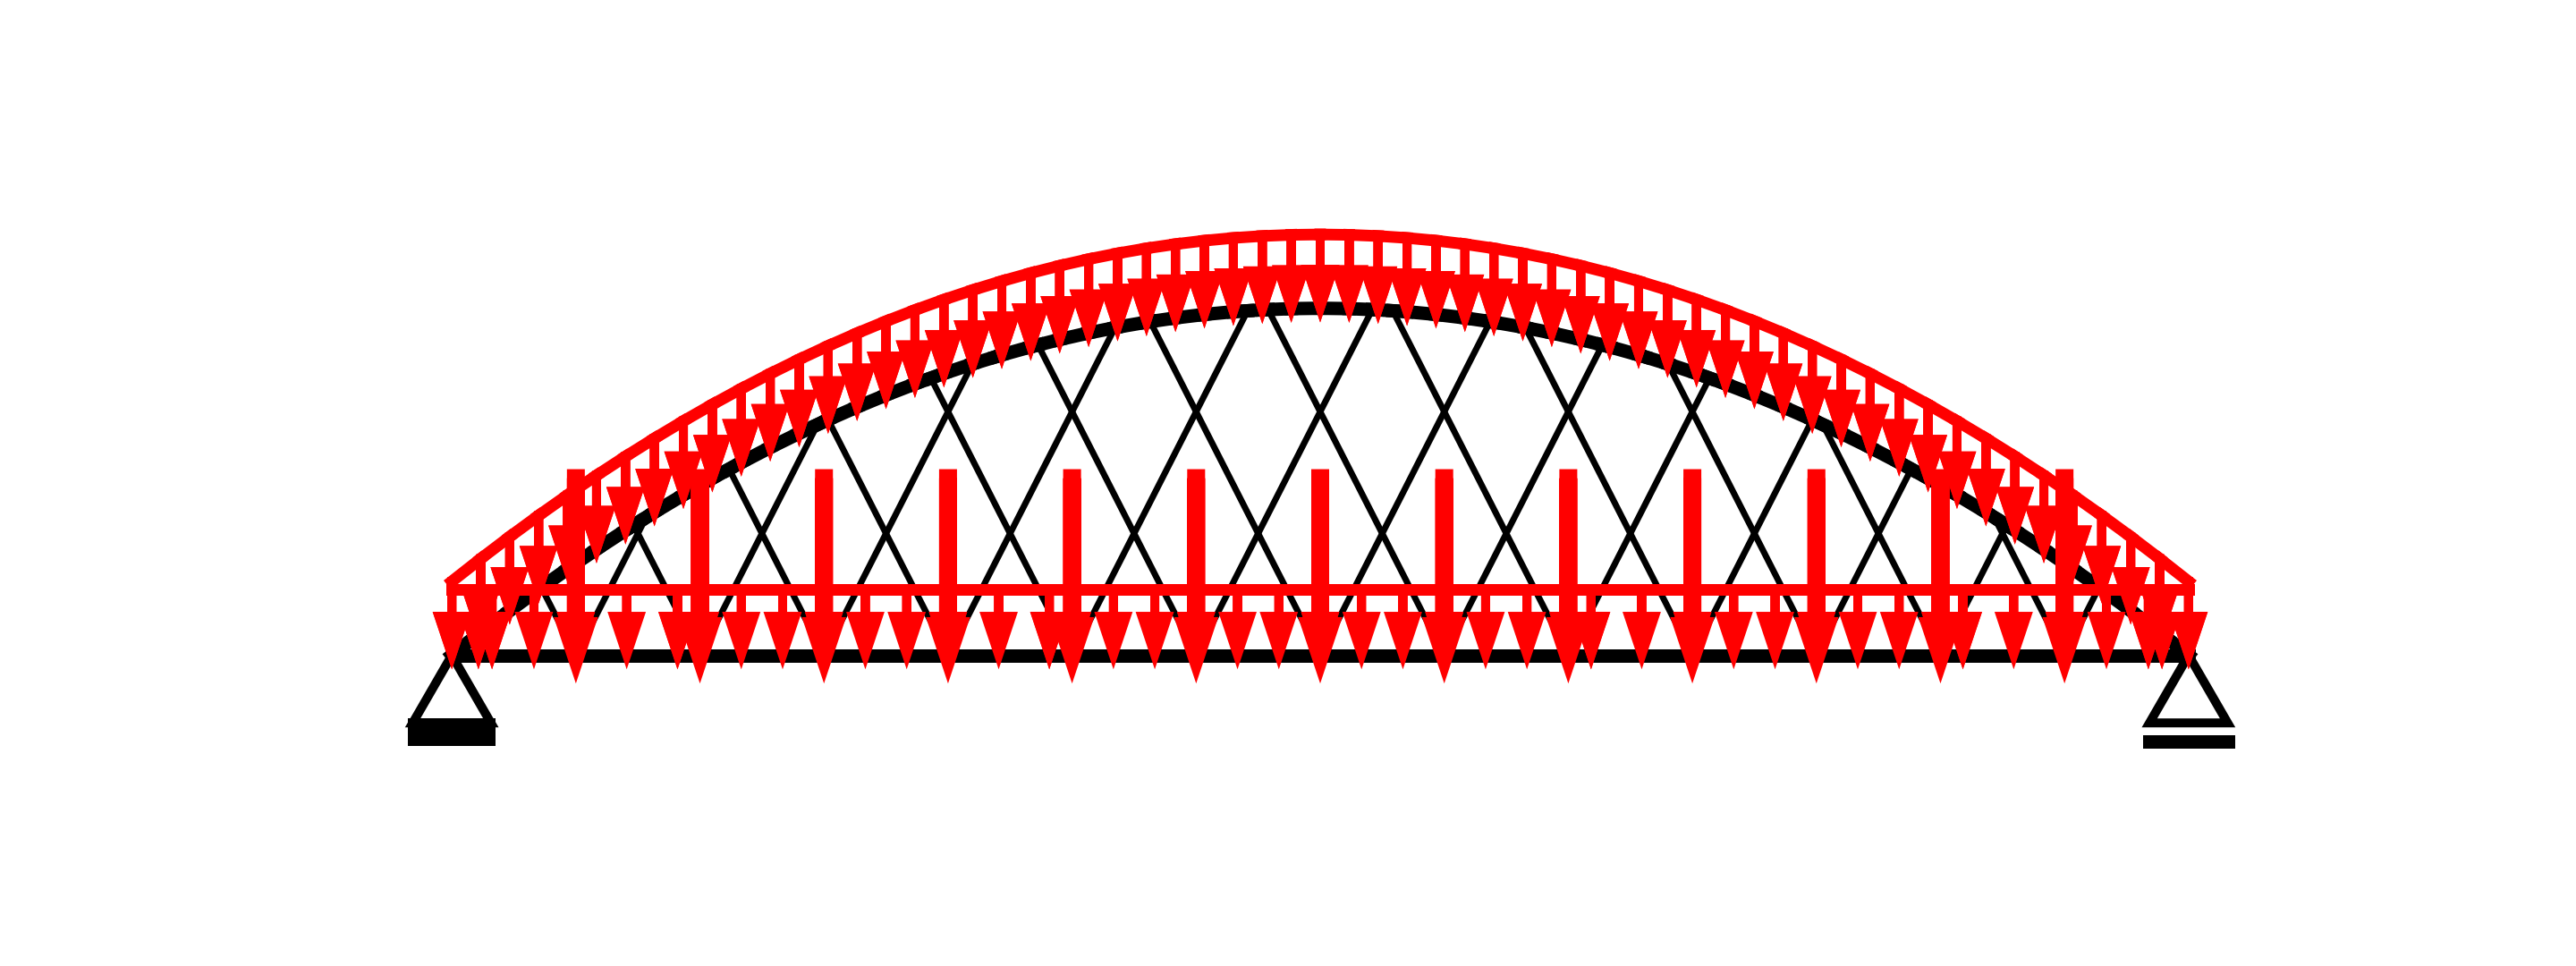
\includegraphics[trim={0 0.8cm 0 0.8cm},clip,
    width=0.8\textwidth]{illustrations/model overview/permanent loads.png}
    \caption{Dead loading in the structural model}
    \label{fig:dead_loads}
\end{figure}

\subsubsection{Live loading}
The load case of live loading is a combination of two separate components. A lane-wise distributed load is applied along the entire or partial length of the bridge and a concentrated truck load is applied at a specific longitudinal point. According to AASHTO code provisions, both loads are factored according to how many lanes they are applied on. Therefore, the number of loaded lanes causing the highest load on one side of the tie girder is determined in a first step. In the detailed calculations in Appendix \ref{Appendx_A_Live_loading} it can be seen that six loaded lanes cause the largest load in one of the arch planes. This conclusion is also valid for the truck loads which are also applied on six lanes. An overview of the design loads is given in Table \ref{tab:live_load_overview}. 

\begin{table}[H]
\centering
\caption{Overview of the live loading}
\label{tab:live_load_overview}
\begin{tabular}{cccccc}
\begin{tabular}[c]{@{}c@{}}Design\\ lane load\end{tabular} & \begin{tabular}[c]{@{}c@{}}Design\\ truck weight\end{tabular} & \begin{tabular}[c]{@{}c@{}}Lane\\ multiplier\end{tabular} & \begin{tabular}[c]{@{}c@{}}Dynamic\\ multiplier\end{tabular} & \begin{tabular}[c]{@{}c@{}}Distributed\\ design load\end{tabular} & \begin{tabular}[c]{@{}c@{}}Concentrated\\ design load\end{tabular} \\ \hline
\SI{9.3}{kN/m} & \SI{325}{kN} & \SI{2.46}{} & \SI{1.33}{} & \SI{23.0}{kN/m} & \SI{1063}{kN}
\end{tabular}
\end{table}


As the live loads are applied on the deck, they act as concentrated forces on the tie at the cross-girders. To find the worst longitudinal arrangement of the live loads, they are applied individually. For each point in the model the partially loaded tie and the concentrated force are combined to produce maximum effects. The concentrated force is thereby only applied at one cross-girder exclusively. It yields a range of possible effects for each point on the structural elements. The resulting ranges for the Blennerhassett Island Bridge are presented in Fig. [], where the ranges of the concentrated load and the distributed loads are also shown individually. These results agree well with the effects specified on the design drawings.


\subsubsection{Wind loading}
The wind load case is not treated in this investigation. However, the effects specified on the design drawing are taken to put results into the context of the integral design. The respective characteristic internal force effects are shown in Table [].

In [] it is mentioned, that the deciding load case for the design of the Blennerhassett Island Bridge is the accidental tie fracture event. It assumes that one of the flanges or the webs of the tie ruptures, which causes immense stresses and strains on the remaining components and also changes the flow of forces. The investigation of this load case lies outside of the scope of this Thesis. Nevertheless, it is indirectly considered in the objective function, which is introduced in Sec. [].

\subsection{Self-equilibrium stress state} \label{sec:met_seq}
% Permanent state

\subsection{Design verifications} \label{sec:met_ver}

\subsection{Estimation of cost function} \label{sec:met_cost}

\begin{table}[H]
\caption{Load combinations for the ultimate limit state}
\centering
\begin{tabular}{lccccc}
\hline
Load         & EL  & DC         & DW         & LL   & WS  \\ \hline
Strength-I   & 1.0 & 0.9 / 1.25 & 0.65 / 1.5 & 1.75 & -   \\
Strength-III & 1.0 & 0.9 / 1.25 & 0.65 / 1.5 & -    & 1.4 \\ 
Strength-IV  & 1.0 & 0.65 / 1.5 & 0.65 / 1.5 & -    & - \\ \hline
\end{tabular}
\end{table}
\begin{table}[H] 
\caption{Effects of wind loading per segment}
\label{tab:effects_wind_load}
\centering
\begin{tabular}{lccc}
\hline
Segment & Normal force & Moment-y & Moment-z \\
 & [MN]   & [MNm] & [MNm] \\ \hline
Arch 1 & -7.8 & -0.67 & 10.7\\
Arch 2 & -4.1 & -0.53 & 2.6\\
Arch 3 & -3.9 & 0.12 & 0.11\\
Tie 1 & 7.0 & -1.1 & 5.9\\
Tie 2 & 6.2 & 0.40 & 0.43\\
Tie 3 & 5.3 & 0.70 & 0.79\\
Hangers & 0.48 & - & - \\ \hline
\end{tabular}
\end{table}

\begin{table}[H] 
\caption{Cross-sectional resistances}
\centering
\begin{tabular}{lccc}
\hline
Segment & Normal force & Moment-y & Moment-z \\
 & [MN]   & [MNm] & [MNm] \\ \hline
Arch 1 & \SI{130.0}{} & \SI{78.7}{} & \SI{79.1}{}\\
Arch 2 & \SI{108.8}{} & \SI{71.5}{} & \SI{63.4}{}\\
Arch 3-4 & \SI{82.3}{} & \SI{50.0}{} & \SI{42.7}{}\\
Tie 1 & \SI{153.2}{} & \SI{100.8}{} & \SI{76.2}{}\\
Tie 2 & \SI{117.1}{} & \SI{82.8}{} & \SI{56.6}{}\\
Tie 3-4 & \SI{100.6}{} & \SI{76.2}{} & \SI{45.8}{}\\
Hangers & 4.19 & - & - \\\hline
\end{tabular}
\end{table}

